% Wczytanie szablonu
\documentclass[nostrict]{Szablon}

% Definicja dokumentu
\usepackage[unicode=true]{hyperref}
\newcommand\PDFtitle{Jak wiele informacji o sobie udostępniamy w Internecie}
\newcommand\PDFauthors{Paulina Brzęcka 184701 Marek Borzyszkowski 184266}
\hypersetup{
  pdftitle={\PDFtitle},
  pdfauthor={\PDFauthors},
}

% \usepackage{textcomp}
\usepackage{array}
% pakiet stosowany do url'i w bibliografii, zamienia odnośniki na ładnie sformatowane
\usepackage{url}
% pakiety służące do numerowania i tworzenia algorytmów
\usepackage{algorithmic}
\usepackage{algorithm}
% redefinicja etykiety nagłówkowej listy algorytmów, domyślna jest po angielsku
\renewcommand{\listalgorithmname}{Spis algorytmów}

% pakiet do wyliczania skali, przydatny przy dużych obrazkach
\usepackage{pgf}
% tworzenie listingów
\usepackage{listings}
% tworzenie figur wewnątrz figur
\usepackage{subfig}

% makro umożliwiające otaczanie symboli okręgami
\usepackage{tikz}
% brak justowania tekstu (bazą okręgu będzie linia tekstu)
\newcommand*\mycirc[1]{%
  \begin{tikzpicture}
    \node[draw,circle,inner sep=1pt] {#1};
  \end{tikzpicture}}

% pionowe justowanie tekstu, środek okręgu pokrywa się ze środkiem tekstu
\newcommand*\mycircalign[1]{%
  \begin{tikzpicture}[baseline=(C.base)]
    \node[draw,circle,inner sep=1pt](C) {#1};
  \end{tikzpicture}}

% zmiana nazwy twierdzeń i lematów
\newtheorem{theorem}{Twierdzenie}[section]
\newtheorem{lemma}[theorem]{Lemat}

% redefinicja dowodu - pogrubiony
\renewenvironment{proof}[1][Dowód]{\begin{trivlist}
\item[\hskip \labelsep {\bfseries #1}]}{\end{trivlist}}
% \newenvironment{definition}[1][Definicja]{\begin{trivlist}
% \item[\hskip \labelsep {\bfseries #1}]}{\end{trivlist}}
% \newenvironment{example}[1][Przykład]{\begin{trivlist}
% \item[\hskip \labelsep {\bfseries #1}]}{\end{trivlist}}
% \newenvironment{remark}[1][Uwaga]{\begin{trivlist}
% \item[\hskip \labelsep {\bfseries #1}]}{\end{trivlist}}

% redefinicja czarnego prostokąta zwyczajowo dodawanego na koniec dowodu - oryginał jest biały
\renewcommand{\qed}{\nobreak \ifvmode \relax \else
      \ifdim\lastskip<1.5em \hskip-\lastskip
      \hskip1.5em plus0em minus0.5em \fi \nobreak
      \vrule height0.75em width0.5em depth0.25em\fi}

% poniższymi instrukcjami można sterować co ma być numerowane a co nie i co ma być wyświetlane w spisie treści
% \setcounter{secnumdepth}{3}
% \setcounter{tocdepth}{5}

% definicja czcionki mniejszej niż tiny (domyślnie takiej małej nie ma)
% \usepackage{lmodern}
\makeatletter
  \newcommand\tinyv{\@setfontsize\tinyv{4pt}{6}}
\makeatother

% definicja jeszcze mniejszej czcionki
% \usepackage{lmodern}
\makeatletter
  \newcommand\tinyvv{\@setfontsize\tinyvv{3.5pt}{6}}
\makeatother

% pakiet do obsługi wielostronicowych tabel
\usepackage{longtable}
\setlength{\LTcapwidth}{\textwidth}

% \usepackage[section] {placeins}

\usepackage{multirow}
\usepackage{booktabs}
\usepackage{slantsc}


% Zmiana czcionki dla symulacji maszynopisu (verbatim)
\makeatletter
\renewcommand{\verbatim@font}{\ttfamily\small}
\makeatother

% Część właściwa pracy
\begin{document}
% 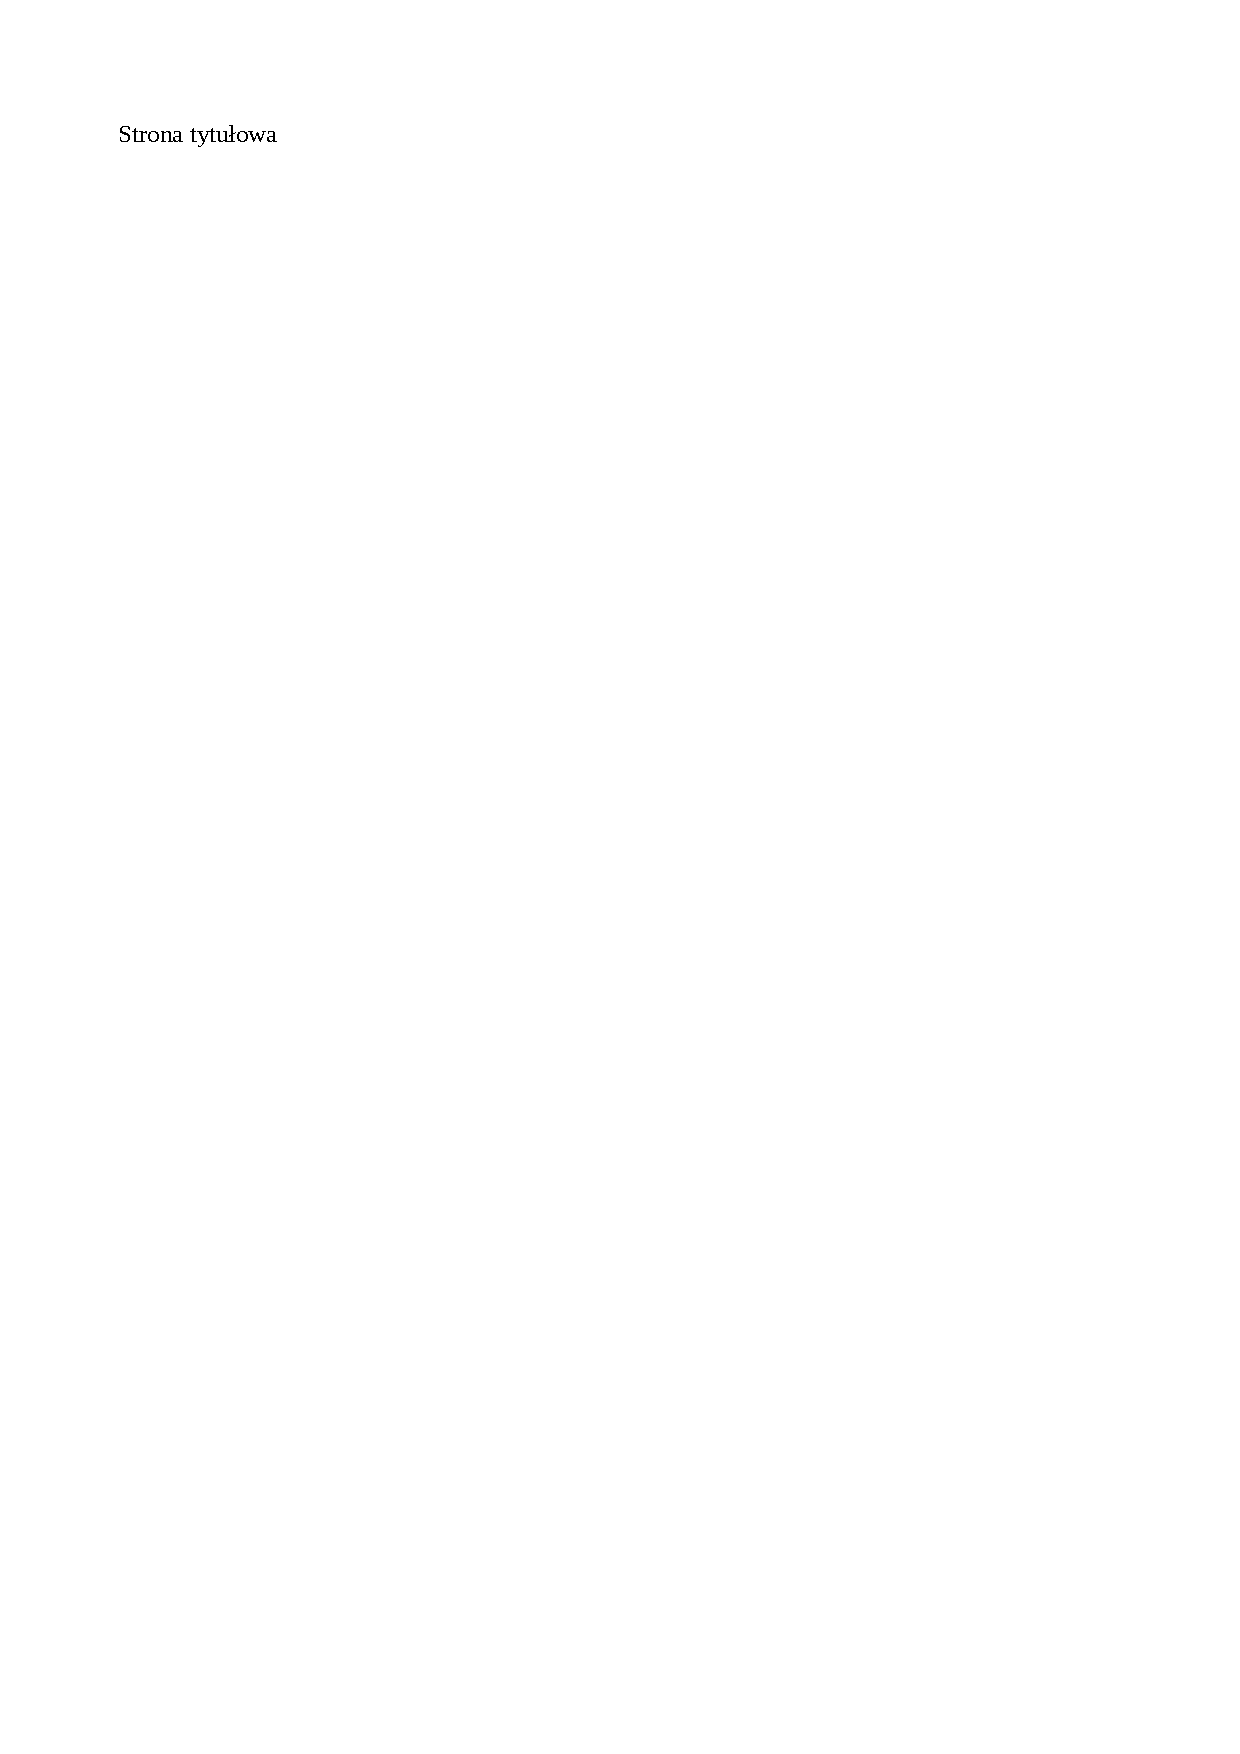
\includepdf{chapters/oswiadczenia/tytulowa.pdf}
% 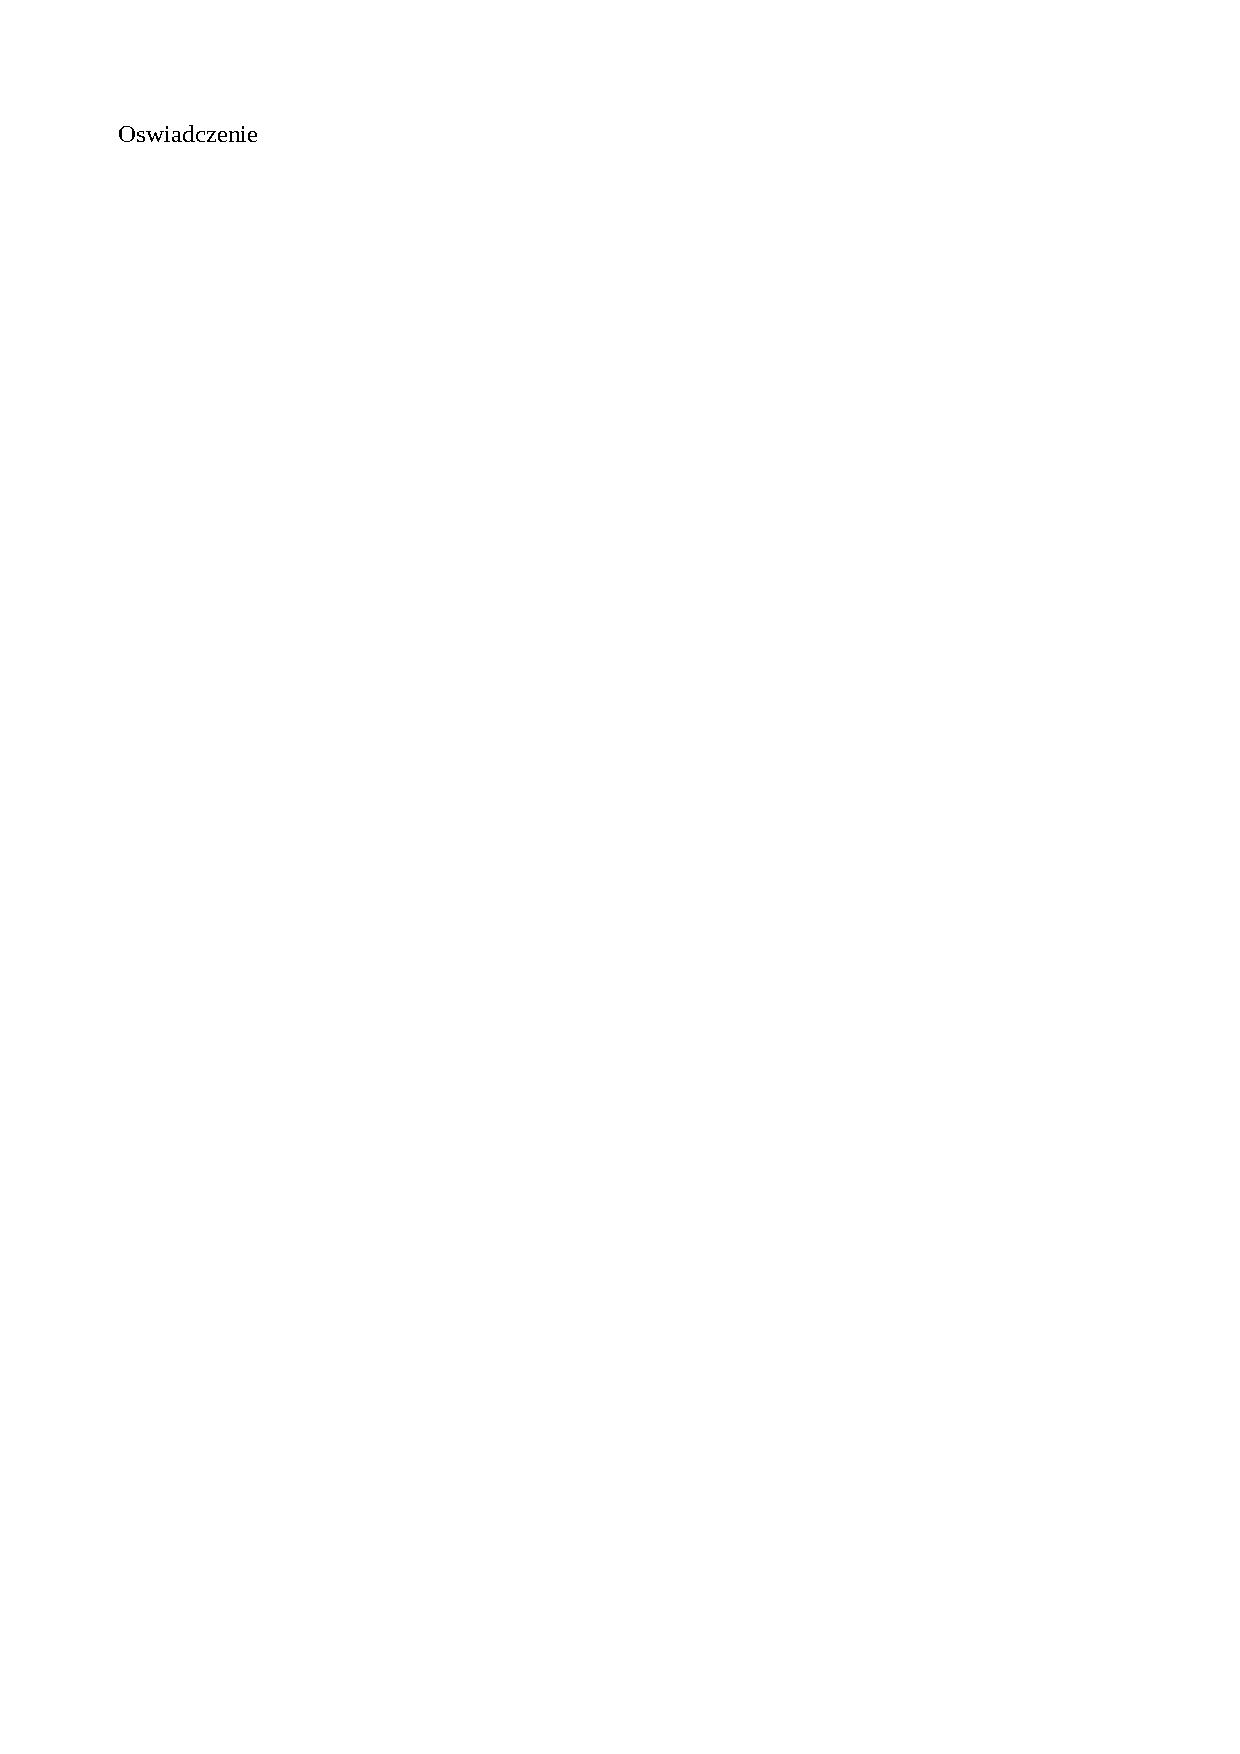
\includepdf{chapters/oswiadczenia/oswiadczenie.pdf}
\title{Jak wiele informacji o sobie udostępniamy w Internecie}
\author{Paulina Brzęcka 184701 Marek Borzyszkowski 184266}
\maketitle
% \hfill
% \pagebreak

% \chapter*{Streszczenie}
% \addcontentsline{toc}{chapter}{STRESZCZENIE}  
Streszczeie ąęśćźżiół
\newline
\newline
\textbf{Słowa kluczowe:} 
Słowo kluczowe 1, Słowo kluczowe 2, Słowo kluczowe 3
\newline
\textbf{Dziedzina nauki i techniki, zgodnie z wymogami OECD: }
\newline
Nauki o komputerach i informatyka


\chapter*{Abstract}
% \addcontentsline{toc}{chapter}{ABSTRACT}  
Abstract in english.
\newline
\newline
\textbf{Keywords:}
Keyword 1, Keyword 2, Keyword 3
\newline
\textbf{Field of science and technology in accordance with OECD requirements: } \newline
Computer Science and Information technology
\addcontentsline{toc}{chapter}{SPIS TREŚCI}
\tableofcontents

% \chapter*{WYKAZ WAŻNIEJSZYCH OZNACZEŃ I SKRÓTÓW}
\addcontentsline{toc}{chapter}{WYKAZ WAŻNIEJSZYCH OZNACZEŃ I SKRÓTÓW}

\textbf{Skrót 1} - Opis 1.


\textbf{Skrót 2} - Opis 2.


\chapter{WSTĘP I CEL PRACY}
\label{chap:introduction}
Wstępu wstępu - tutaj należy pokrótce opisać o co chodzi w pracy i wyraźnie wskazać cel pracy!
% \begin{figure}[H]
%     \centering
%     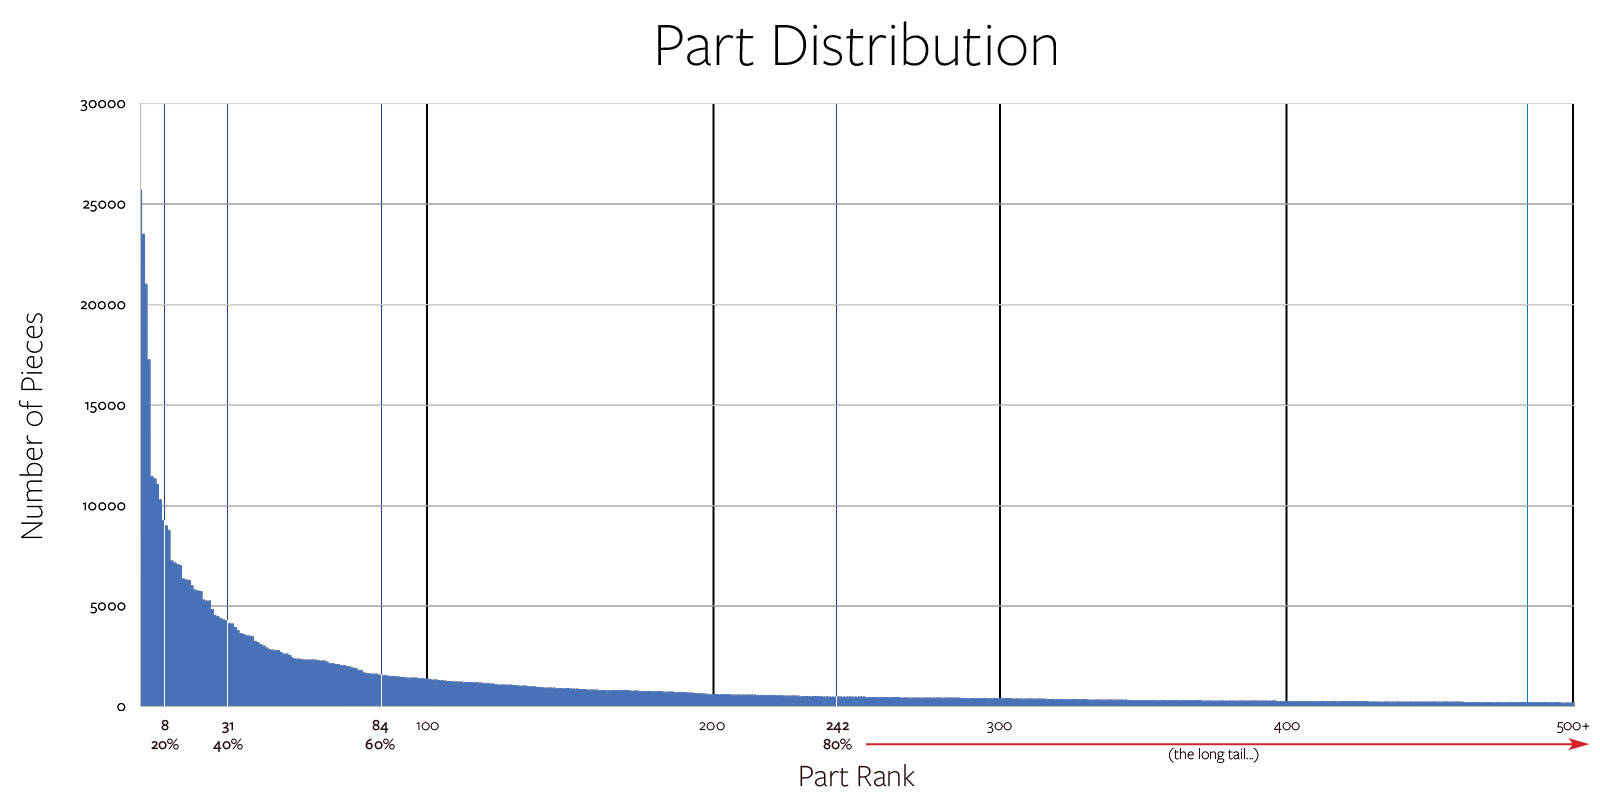
\includegraphics[width=1\textwidth]{images/part_dist.jpg}
%     \caption{Szacunkowa dystrybucja klas klocków kupionych w latach 2015-2020\cite{dist}}
%     \label{fig:part_dist}
% \end{figure}
% Na wykresie \ref{fig:part_dist} terefere.
\section{Cel pracy}
Mój super cel. 
\section{Układ pracy}
Układ pracy jest następujący...


\chapter{ANALIZA PODSTAWOWYCH DANYCH I BUDOWA PROFILU}

To jest rozdział.

\section{Podrozdziały}

W Latexu w klasie dokumentów \textbf{book} wyróżniamy rozdziały (\textbf{chapter}), podrozdziały \textbf{section}, podpodrozdziały \textbf{subsection}, podpodpodrozdziały \textbf{subsubsection} i paragrafy (\textbf{paragraph}). Podpodpodrozdziały i paragrafy domyślnie nie są numerowane ani nie występują w spisie treści. Zachowanie to można zmienić poprzez funkcję \textbf{setcounter} umieszczaną w preambule. Wykomentowany przykład można znaleźć w kodzie tego dokumentu.

Obecnie znajdujemy się na poziomie podrozdziału. Pozostałe przykłady poniżej.

\subsection{Podpodrozdział}

To jest podpodrozdział.

\subsubsection{Podpodpodrozdział}

To jest podpodpodrozdział. On nie jest domyślnie numerowany i nie występuje w spisie treści.

\paragraph{Paragraf}

A to jest paragraf. On również nie jest domyślnie numerowany i nie występuje w spisie treści.

\section{Podstawowe elementy typograficzne}

\subsection{Twarda spacja}

Twarda spacja jest bardzo istotnym elementem, gdyż zabrania Latex'owi łamanie linii w miejscu jej wystąpienia, a tym samym pozwoli na niejako ,,sklejenie'' wyrazów ze sobą. Dzięki temu możemy uniknąć tzw.\ sierot (pojedynczych znaków na końcu wiersza). W Latex twardą spację umieszcza się wstawiając znak tyldy~(\textasciitilde). Zapisujemy to więc np.\ tak: ,,dokument, w{\textasciitilde}którym''.

\subsection{Formatowanie tekstu}

Aby zapewnić poprawny wygląd tekstu należy pamiętać o kilku rzeczach:

\begin{itemize}
 \item Linia poprzedzona procentem to komentarz.
 \item Poprzedzaniu spacji występującej po kropce kończącej skrót znakiem ucieczki, odstęp będzie wtedy taki, jak odstęp między wyrazami a~nie między zdaniami. Przykładowo zapis ,,np. tekst'' vs. ,,np.\ tekst''. Ten drugi jest poprawny, a zapisany został tak: ,,np.$\backslash$~tekst''.
 \item Skróty pisane wielkimi literami kończące zdanie powinny posiadać {$\backslash$}@ przed kropką kończącą zdanie, np.\ OCS{$\backslash$}@\@. Spowoduje to potraktowanie spacji jako spacji międzyzdaniowej z nie międzywyrazowej.
 \item Cudzysłowie zawsze tworzymy używając podwójnego przecinka jako symbolu otwierającego cudzysłów, oraz podwójnego apostrofu zamykającego cudzysłów.
 \item Kursywę uzyskujemy za pomocą słowa kluczowego {$\backslash$}textit, co w efekcie daje \textit{tekst kursywą}. Pogrubiony \textbf{używamy słowa kluczowego textbf}. Każdorazowo tekst mający być napisany danym krojem otaczamy nawiasami klamrowymi.
 \item Myślnik (--) tworzymy poprzez umieszczenie bezpośrednio po sobie dwu kresek (minusy). Różnica między nimi jest zasadnicza. Pojedynczy myślnik generuje krótką kreskę (-), podwójny długą (--), potrójny najdłuższą (---).
 \item Odwołania do różnych elementów dokumentu robimy poprzez słowo kluczowe \textbf{ref()}. Jako jego parametr wstawiamy nazwę zdefiniowaną za pomocą słowa kluczowego \textbf{label()}. Należy pamiętać, że odwołanie zwraca jedynie numer elementu, słowo opisowe, jak np.\ rozdział czy rysunek należy dodać samodzielnie. Polecam tutaj przyjąć jakąś konwencję i się jej trzymać w całym dokumencie. Tak samo należy postępować w przypadku etykiet.
 \item Latex doskonale radzi sobie z dzieleniem wyrazów na końcach linii, jednak czasami zachodzi konieczność wymuszenia podziału w określonym miejscu. W tym celu należy zastosować konstrukcję $\backslash$-. Latex takiego ukośnika nie wydrukuje dopóty, dopóki rzeczywiście w tym miejscu nie zostanie wykonane przeniesienie części wyrazu. Możliwe jest dodanie wielu podziałów w jednym wyrazie. Użyte wtedy zostanie to, które spowoduje wygenerowania ,,najładniejszego'' tekstu.
\end{itemize}

\section{Podział linii i paragrafy}
% \label{podzial}

Nowy paragraf rozpoczyna się poprzez wstawienie jednej wolnej linii. Latex automatycznie wygeneruje wcięcie. Należy pamiętać, że pierwszy paragraf, zgodnie ze standardami drukarskimi, nie ma wcięcia! Możemy tym sterować za pomocą poleceń \textbf{noindent} (brak wcięcia) oraz \textbf{indent} (dodatkowe wcięcie).

Jeżeli chcemy po prostu zrobić nową linię, bez tworzenia nowego paragrafu używamy konstrukcji $\backslash\backslash$. Efekt będzie taki, że paragraf\\
będzie kontynuowany w nowej linii. Nie spowoduje to jednak rozciągnięcia poprzedniej linii. Zostanie ona przerwana tam gdzie tego sobie zażyczymy i kontynuowana w nowej linijce.

A co w przypadku, gdy chcemy z jakiegoś powodu przerwać linię, ale wymusić justowanie tekstu? Weźmy dla przykładu fragment:

Trzecim istotnym aspektem jest stosowana w~trakcie wytwarzania ontologii metodologia pracy~\cite{boinski2012kaskbook,boinski2011security}. Zastosowanie jednej z~uznawanych metodologii, takich jak Methontology, NeOn czy metodologia opracowana przez Noy~i~McGuiness, znacząco wpływa na jakoś uzyskanego produktu. Wspomniane metodologie w~dużej mierze uwzględniają potrzebę przyszłej integracji wiedzy, a~w połączeniu z~narzędziami typu Protégé czy OCS~\cite{boinski2007kaskbook,boinski2009ocs,boinski2010zespolowa}, pozwalają na tworzenie spójnych i~formalnie oraz logicznie poprawnych ontologii.

Tekst zostaje bardzo brzydko złamany w środku odnośników do cytowań. Użycie podwójnego po słowie ,,metodologia'' w pierwszym zdaniu ukośnika da nam natomiast taki efekt:

Trzecim istotnym aspektem jest stosowana w~trakcie wytwarzania ontologii metodologia \\ pracy~\cite{boinski2012kaskbook,boinski2011security}. Zastosowanie jednej z~uznawanych metodologii, takich jak Methontology, NeOn czy metodologia opracowana przez Noy~i~McGuiness, znacząco wpływa na jakoś uzyskanego produktu. Wspomniane metodologie w~dużej mierze uwzględniają potrzebę przyszłej integracji wiedzy, a~w połączeniu z~narzędziami typu Protégé czy OCS~\cite{boinski2007kaskbook,boinski2009ocs,boinski2010zespolowa}, pozwalają na tworzenie spójnych i~formalnie oraz logicznie poprawnych ontologii.

Też nie ładnie, gdyż linijka jest niewyjustowana. Z pomocą przychodzi nam tutaj komenda \textbf{linebreak[]}, gdzie w nawiasie kwadratowym podajemy liczbę od 1 do 4 określająca jak bardzo zależy nam na tym, by linia została złamana w tym miejscu (4 to najwyższa wartość). Efekt jest następujący:

Trzecim istotnym aspektem jest stosowana w~trakcie wytwarzania ontologii metodologia \linebreak[4] pracy~\cite{boinski2012kaskbook,boinski2011security}. Zastosowanie jednej z~uznawanych metodologii, takich jak Methontology, NeOn czy metodologia opracowana przez Noy~i~McGuiness, znacząco wpływa na jakoś uzyskanego produktu. Wspomniane metodologie w~dużej mierze uwzględniają potrzebę przyszłej integracji wiedzy, a~w połączeniu z~narzędziami typu Protégé czy OCS~\cite{boinski2007kaskbook,boinski2009ocs,boinski2010zespolowa}, pozwalają na tworzenie spójnych i~formalnie oraz logicznie poprawnych ontologii.

Jeżeli z jakiegoś powodu potrzebujemy nową linię to używamy komendy \textbf{newpage}. \newpage Tekst występujący po niej znajdzie się na nowej stronie. Rozdziały itp.\ automatycznie generują nową stronę, przy czym w układzie dwustronnym nowy rozdział zawsze zacznie się od nieparzystej strony.

\section{Środowisko matematyczne}

Środowisko matematyczne otwieramy i zamykamy znakiem \$. Niektóre funkcje można używać tylko wewnątrz takiego środowiska. Przykładem niech będzie funkcja \textbf{mathcal} zamieniająca duże litery w symbole o charakterystycznym kroju, stosowanym do opisywania stałych, np.\ $\mathcal{O}$ czy $\mathcal{R(D,P,T,S,U,I)}$. Pamiętać należy, że zamienione zostaną wszystkie litery w wyrażeniu występującym wewnątrz nawiasów klamrowych.

Niektóre konstrukcje, np.\ równania, automatycznie włączają tryb matematyczny. Równania dobrze jest opisać, przykład przedstawia Równanie~\ref{eq:przyklad}.

\begin{equation}
  \mathcal{O(K,B,C,R)}
  % \label{eq:przyklad}
\end{equation}

gdzie:\\
$\mathcal{K}$ - zbiór klas wchodzących w~skład ontologii,\\
$\mathcal{B}$ - zbiór bytów wchodzących w~skład ontologii,\\
$\mathcal{C}$ - zbiór komentarzy przypisanych do klas $\mathcal{K}$ i~bytów $\mathcal{B}$ wchodzących w~skład ontologii,\\
$\mathcal{R}$ - zbiór relacji wiążących elementy ontologii.


W równaniach możemy stosować różne dodatkowe symbole oraz np.\ wyrównywać je do określonego miejsca. Służy do tego blok typu \textbf{split}, a sam punkt wyrównania określony jest ampersandem (\&). Przykład zastosowania prezentuje równanie~\ref{eq:split_ex}.

\begin{equation}
  % \label{eq:split_ex}
  \begin{split}
    \forall {x_1 \leq y_1, x_2 \leq y_2}&: f(x_1+x_2,y_1+y_2)\\ 
				  &= \frac{y_1}{y_1+y_2}f(x_1,y_1)+\frac{y_2}{y_1+y_2}f(x_2,y_2)
  \end{split}
\end{equation}

\subsection{Twierdzenia i dowody}

Linie 75 -- 93 nagłówka dokumentu definiują nowe nazwy sekcji twierdzeń i dowodów, oraz znacznik końca dowodu (taki czarny kwadracik). Dzięki nim można uzyskać ładnie wyglądające twierdzenia jak poniżej (Twierdzenie~\ref{eq:lin:theorem}). Zauważmy, że równanie dowodu nie jest równaniem numerowanym. Wszędzie tam, gdzie nie chcemy by rozdział czy dowolna inna sekcja była numerowana należy w jej nazwie użyć gwiazdki, np. \textbf{$\backslash$begin\{equation*\}}.

\begin{theorem}
 Podobieństwo pomiędzy pojęciami $A$ i~$B$ opisane jest stosunkiem ilości informacji niezbędnej do opisania ich wspólności znaczeniowej oraz ilością informacji niezbędnej do ich opisania (Równanie~\ref{eq:lin:theoremeq}).

 \begin{equation}
   sim_{lin}(A,B)=\frac{\log P(common(A,B))}{\log P(description(A,B))}
  %  \label{eq:lin:theoremeq}
 \end{equation}
%  \label{eq:lin:theorem}
\end{theorem}

\begin{proof}
  \begin{equation*}
   \begin{split}
     f(x,y)&=f(x+0,y+(y-x))\\
	   &=\frac{x}{y}*f(x,x) +~\frac{y-z}{x}*f(0,y-z)\\
	   &=\frac{x}{y}*1 +~\frac{y-z}{x}*0\\
	   &=\frac{x}{y} \qed
   \end{split}
 \end{equation*}
\end{proof}

Inna ciekawa konstrukcja wykorzystująca tryb matematyczny do zapisania pewnego stwierdzenia:

Niech $A \subseteq T$, $C = N_y(A) \neq W$, a~$\alpha_y = \min_{a \in A, b\notin C} \{y(a) +~y(b) - q(a, b)\}$ oraz

\[ y'(v) = \left\{ \begin{array}{ll}
                y(v) - \alpha_y & \mbox{jeżeli $v \in A$} \\
                y(v) +~\alpha_y & \mbox{jeżeli $v \in C$} \\
                y(v)            & \mbox{w innych przypadkach}
               \end{array}
       \right. \]

Zapis ten, acz skomplikowany, pozwala na reprezentację złożonych reguł matematycznych w postaci ładnie ułożonych i wyrównanych wierszy. Reguły \textbf{left} oraz \textbf{right} pozwalają na utworzenie nawiasów klamrowych, których rozmiar będzie automatycznie dostosowywany do rozmiaru elementu, jakie mają zawierać.

\chapter{ŹRÓDŁA POZYSKIWANIA INFORMACJI}
\enlargethispage{20pt}

\section{Identyfikacja i analiza publicznie dostępnych źródeł}

W dobie powszechnego dostępu do Internetu oraz ogromnej popularności mediów społecznościowych, zdobycie informacji na temat osoby prywatnej, przedsiębiorcy czy pracownika jest dziś łatwiejsze niż kiedykolwiek wcześniej. Użytkownicy często sami - świadomie lub nieświadomie - pozostawiają po sobie szereg danych, które można wykorzystać do stworzenia precyzyjnego profilu.

Według raportu „Digital 2021” (We Are Social i Hootsuite), z Internetu w Polsce korzysta 31,97 mln osób, a 25,9 mln aktywnie używa mediów społecznościowych. To oznacza, że większość społeczeństwa codziennie generuje cyfrowe ślady, które mogą być później analizowane.\cite{zrodlo}

\subsection{Media społecznościowe}

Facebook, Instagram, X, LinkedIn czy Snapchat gromadzą dane zarówno świadomie podawane przez użytkowników (np. miejsce pracy), jak i te zbierane automatycznie - lokalizacja, adres IP, urządzenia.
Dane mogą pochodzić także z aplikacji firm trzecich, programów lojalnościowych czy partnerów marketingowych.\cite{zrodlo2}

Szczegółowe zestawienie, jakie dane są gromadzone w mediach społecznościowych zostały przedstawione w poniższej tabeli. \cite{zrodloArtykul}
\begin{longtable}{p{8.5cm}|c|c|c}
\toprule
\textbf{Zakres danych / Działanie} & \textbf{Facebook} & \textbf{X} & \textbf{LinkedIn} \\
\midrule
\multicolumn{4}{l}{\textbf{DANE OSOBOWE}} \\
Imię i nazwisko & + & + & + \\
E-mail & + & + & + \\
Numer telefonu & + & + & + \\
Data urodzenia & + & + & + \\
Adres zamieszkania & + & + & + \\
Poprzednie miejsca zamieszkania & + &  &  \\
Zdjęcia profilowe & + & + & + \\
Rodzina i związki & + &  &  \\
Wykształcenie & + &  & + \\
Języki obce & + &  & + \\
Poglądy polityczne & + &  &  \\
Przekonania religijne & + &  &  \\
Wydarzenia z życia & + &  &  \\
\midrule
\multicolumn{4}{l}{\textbf{DANE ZAWODOWE I LOKALIZACYJNE}} \\
Miejsce pracy & + &  & + \\
Kwalifikacje & + &  & + \\
Wynagrodzenie &  &  & + \\
Płatności & + &  & + \\
Lokalizacja & + & + & + \\
Urządzenia & + & + & + \\
Adres IP & + & + & + \\
Kalendarz &  &  & + \\
\midrule
\multicolumn{4}{l}{\textbf{ŹRÓDŁA POZYSKIWANIA INFORMACJI}} \\
Od użytkownika & + & + & + \\
Od innych użytkowników & + & + & + \\
Od partnerów zewnętrznych & + &  & + \\
Z aplikacji zewnętrznych & + & + &  \\
Z aktywności (kliknięcia) & + & + &  \\
\midrule
\multicolumn{4}{l}{\textbf{ZASTOSOWANIA I UDOSTĘPNIANIE}} \\
Reklamy & + & + & + \\
Personalizacja & + & + & + \\
Oznaczanie na zdjęciach & + &  &  \\
Meldowanie w lokalizacjach & + & + &  \\
Sugestie kontaktów & + &  & + \\
Udostępnianie firmom & + & + & + \\
Cele badawcze i analityczne & + & + & + \\
\bottomrule
\end{longtable}

Jesli chodzi o Facebook, to gromadzi on najszerszy zakres danych - zarówno prywatnych, jak i zawodowych, w tym dane kontaktowe, lokalizacyjne, relacyjne i behawioralne. Dane są również pozyskiwane od partnerów i aplikacji zewnętrznych. Warto zaznaczyć, że domyślne ustawienia prywatności, których większość użytkowników nigdy dokładnie nie czyta przed akceptacją, bardzo często sprzyjają upublicznieniu informacji, a około 40\% użytkowników nie zmienia nigdy ustawień prywatności, co czyni ich dane łatwo dostępnymi.

W aplikacji X domyślnie wszystkie posty (tweety) są publiczne. Dodatkowo dane gromadzone również poprzez partnerów i aplikacje zewnętrzne, a polityka firmy jest dosyć liberalna i udostępnia dane badaczom.

Firma LinkedIn dodatkowo profiluje użytkowników głównie pod kątem danych zawodowych (miejsce pracy, kwalifikacje, języki), które potem są wykorzystywane komercyjnie i sprzedawane firmom rekrutacyjnym. Może być to szczególnie niebezpieczne przy atakach typu spear-phishing, gdzie precyzyjne informacje są używane do podszywania się i oszustw.

\subsection{Fora, sekcje komentarzy, blogi}

Uznawane za „anonimowe”, w rzeczywistości łatwe do deanonimizacji. Powtarzające się pseudonimy, zdjęcia profilowe, adresy IP - wszystko to pozwala powiązać konto z konkretną osobą, po mniej lub bardziej wnikliwym poszukiwaniu.

\subsection{Rejestry publiczne i portale firmowe}
Z racji powszechnej cyfryzacji, przed udostępnieniem niektórych danych w internecie nie można się uchronić. Szczególnie osoby prowadzące firmy lub działalności gospodarcze, a nawet osoby posiadające nieruchomości. 
Nie wspominając o tym, że prawie każdy dorosły człowiek w dzisiejszych czasach pracuje w jakiejś firmie, gdzie często dane kontaktowe, adresy e-mail, a czasem także numery telefonów pracowników czy właścicieli firm są udostępniane na stronie firm, bardzo często nawet bez wiedzy samych zainteresowanych.\cite{zrodloDzialalnosc} \\
Niektóre dane są dostępne w postaci rejestrów internetowych:

\begin{itemize}
  \item \textbf{CEIDG} - zawiera dane o jednoosobowej działalności gospodarczej, w tym adres, który nierzadko jest miejscem zamieszkania. 
  \item \textbf{KRS} - dane zarządu, często z numerem PESEL, umożliwia pozyskanie numeru PESEL i daty urodzenia członków zarządu spółek.
  \item \textbf{CRBR} - udostępnia dane beneficjentów rzeczywistych, w tym numery PESEL udziałowców spółek.
  \item \textbf{Elektroniczne Księgi Wieczyste} - umożliwiają dotarcie do danych właścicieli nieruchomości.
  \item \textbf{Portale ogłoszeniowe, firmowe} - e-maile, telefony, nazwiska
\end{itemize}

\subsection{Urządzenia IoT}

Inteligentne urządzenia domowe (głośniki, żarówki, lodówki) zbierają dane o rutynie, lokalizacji i obecności użytkownika. Coraz więcej urządzeń domowych (np. tostery, żarówki, głośniki) jest wyposażanych w moduły internetowe. Nawet jeśli nie oferują realnych funkcji online, dane z nich są zbierane i mogą być wykorzystywane marketingowo. Koszt wdrożenia łączności IoT dla producenta jest niewielki, a dane mają wysoką wartość.

\begin{quote}
„Kupując sprzęt domowy, możemy nieświadomie nabyć urządzenie IoT. Kluczowym zasobem są dane - które mogą zostać sprzedane lub wykorzystane przez producenta.” - Mikko Hypponen
\end{quote}

\subsection{Czat AI jako nieświadome źródło informacji}
Coraz więcej osób korzysta z narzędzi opartych na sztucznej inteligencji (AI), takich jak ChatGPT czy Bing Chat, aby wspierać się w pracy zawodowej. Według badań aż 43\% pracowników używa AI do realizacji swoich zadań.\cite{ai} Choć AI oferuje wygodne i szybkie odpowiedzi, istnieją zagrożenia dotyczące prywatności i bezpieczeństwa danych, o których warto pamiętać, że:

\begin{itemize}
  \item dane mogą być przetwarzane lub analizowane przez ludzi,
  \item platformy zastrzegają prawo do przechowywania zapytań,
  \item AI modele, takie jak ChatGPT, mogą uczyć się na podstawie zadawanych pytań. Dlatego nie powinno się wprowadzać do nich żadnych danych osobowych ani poufnych.
\end{itemize}

\textbf{Co zdarza się ludziom udostępnić, a nie powinno się tego robić:}

\begin{itemize}
  \item Imię i nazwisko,
  \item Data urodzenia,
  \item Adres zamieszkania,
  \item Numer dowodu osobistego,
  \item Telefon, adres e-mail,
  \item Kod źródłowy lub dane z projektów w fazie rozwoju,
  \item Poufne informacje o produktach i usługach,
  \item Niezaprezentowane jeszcze pomysły lub rozwiązania,
  \item Numery kart kredytowych,
  \item Numery kont bankowych,
  \item Hasła i dane logowania,
  \item Wyniki badań,
  \item Diagnozy lekarskie,
  \item Informacje dotyczące leczenia.
\end{itemize}

\textbf{Aby korzystać z AI w sposób odpowiedzialny i bezpieczny, warto stosować się do kilku prostych zasad:}

\begin{itemize}
  \item Używanie jedynie informacji ogólnodostępnych i nieidentyfikujących,
  \item Podawanie dane fikcyjne lub zanonimizowane, jeśli konieczne jest podanie przykładu.
  \item Nie publikowanie szczegółowych planów podróży lub wakacji — może to narażać na kradzież lub inne ryzyko offline.
  \item Założenie drugiego, anonimowego konta, które nie jest powiązane z właściwą tożsamością.
  \item Korzystanie z bezpiecznego połączenia internetowego — unikanie otwartych sieci Wi-Fi w kawiarniach czy hotelach.
  \item Nie udostępnianie haseł ani nie proszenie AI o ich generowanie na potrzeby konkretnej usługi.
  \item Zachowanie ostrożności przy danych zdrowotnych, finansowych i prywatnych,
  \item Zapoznanie się z regulaminem i polityką prywatności chatu AI,
  \item Sprawdzenie, jakie dane są przechowywane, jak długo i komu mogą być udostępniane,
  \item Zwrócenie uwagi, czy narzędzie przewiduje możliwość przeglądu zapytań przez człowieka w celach jakościowych.
\end{itemize}

\section{W jaki sposób dane trafiają w niepowołane ręce?}
Chociaż skoro myślimy, że udostepniamy bardzo mało danych, bądź wcale, istnieją aktualnie techniki, które są na tyle zaawansowane, że na podstawie jednej, bądź kilku informacji można stworzyć czyiś profil osobowy. Do jednej z nich zalicza się biały wywiad. 
Open Source Intelligence, cyli biały wywiad, to wyspecjalizowana technika polegająca na analizie dostępnych publicznie informacji w celu identyfikacji i gromadzenia danych o wybranej osobie.

\begin{itemize}
  \item przeszukiwanie stron internetowych pod kątem danych kontaktowych,
  \item wyszukiwanie kont społecznościowych na podstawie adresu e-mail lub loginu,
  \item analizę zdjęć w celu rozpoznania wizerunku i odnalezienia powiązanych treści,
  \item korelowanie fragmentarycznych danych z różnych źródeł (np. fora, blogi, komentarze).
\end{itemize}

Aktualne narzędzie umożliwiają bardzo wnikliwą analizę, między innymi:

\begin{itemize}
  \item automatyczne przeszukiwanie domen internetowych w celu odnalezienia adresów e-mail,
  \item sprawdzanie, na jakich portalach społecznościowych zarejestrowano konkretne nazwy użytkowników,
  \item analizę zdjęć za pomocą sztucznej inteligencji w celu identyfikacji osoby.
\end{itemize}

Chociaż prawda jest taka, że nie potrzeba żadnych profesjonalnych narzędzi, aby komuś uprzykrzyć życie. Dostęp do danych wrażliwych może mieć każda osoba prywatna, wystarczy tylko odrobina negatywnej motywacji oraz chwila czasu spędzona na poszukiwaniu i wnioskowaniu, ale o tym wiecej w nastepnych rozdziałach. 
\chapter{WYKORZYSTANIE DANYCH PRZEZ RÓŻNE PODMIOTY}

\noindent
Współcześnie informacje gromadzone na temat użytkowników Internetu stały się \textbf{strategicznym zasobem} w wielu branżach. Dane te mogą być wykorzystywane zarówno w legalnych i powszechnie akceptowanych procesach biznesowych, jak i w działaniach sprzecznych z prawem oraz zasadami etyki. W niniejszym rozdziale omówiono główne kierunki wykorzystania danych przez różnorodne podmioty, ze szczególnym uwzględnieniem sektora reklamowego, firm rekrutacyjnych oraz środowiska cyberprzestępców.

\vspace{1em}

\section{Firmy reklamowe i sektor marketingu}

\subsection{Personalizacja i targetowanie reklam}
Dynamiczny rozwój platform cyfrowych umożliwił firmom reklamowym gromadzenie i przetwarzanie ogromnych ilości danych, takich jak:
\begin{itemize}
    \item \emph{historia przeglądania stron internetowych},
    \item \emph{aktywność w mediach społecznościowych},
    \item \emph{dane transakcyjne} (np. preferencje zakupowe, częstotliwość dokonywania zakupów online).
\end{itemize}
Jak podkreśla raport \emph{Behind the One-Way Mirror} opublikowany przez EFF\cite{EFF}, tak szeroki zakres informacji pozwala na \textbf{targetowanie behawioralne}, w którym reklamy są dopasowywane do konkretnych grup odbiorców, uwzględniając ich indywidualne cechy i preferencje.

W praktyce oznacza to, że użytkownikowi, który często wyszukuje informacje o zdrowym stylu życia, mogą się wyświetlać reklamy związane z dietą i aktywnością fizyczną. Natomiast osoby zainteresowane planowaniem podróży będą otrzymywać propozycje ofert turystycznych. Mechanizm ten, choć zwiększa \emph{trafność} komunikatów marketingowych, jednocześnie - jak wskazują liczne analizy rynkowe - \textbf{podnosi} skuteczność kampanii reklamowych i skłania użytkowników do częstszych interakcji z treściami sponsorowanymi.

\subsection{Wykorzystanie Big Data w analizie zachowań konsumenckich}
Zgodnie z danymi statystycznymi przywoływanymi w raporcie \emph{Digital 2025 Global Overview Report}\cite{DIGITAL_GLOBAL}, liczba użytkowników Internetu stale rośnie, a firmy reklamowe i agencje marketingowe mogą dzięki temu gromadzić coraz bardziej rozbudowane zasoby Big Data. Informacje o ścieżkach zakupowych czy upodobaniach pozwalają:
\begin{itemize}
    \item \textbf{segmentować} odbiorców według wielu kryteriów (np. styl życia, wiek, dochód),
    \item \textbf{przewidywać} zachowania (np. kto najchętniej dokona zakupu w danej kategorii produktów),
    \item \textbf{monitorować} skuteczność kampanii w czasie rzeczywistym.
\end{itemize}

Takie dane służą również do tworzenia \emph{dynamiki cenowej} (tzw. \emph{price discrimination}), gdzie użytkownicy otrzymują zindywidualizowane oferty w zależności od historii wyszukiwań i wcześniejszych interakcji z reklamami. Dzięki temu możliwe jest zwiększanie zysków firm, ale pojawiają się też wątpliwości etyczne co do stopnia ingerencji w prywatność konsumentów.

\subsection{Nowe formaty reklamowe i ekosystem wymiany danych}
Raporty dotyczące rynku cyfrowego wskazują, że w obszarze marketingu zachodzi \emph{przesunięcie} z tradycyjnych form reklamy (banery, wyskakujące okienka) w stronę treści natywnych oraz tzw. \textbf{mikro-targetowania}. W tym procesie kluczową rolę pełnią:
\begin{itemize}
    \item \textbf{wielkie platformy internetowe} (np. Google, Facebook, TikTok), które gromadzą i scalają dane o aktywnościach użytkowników,
    \item \textbf{agencje analityczne} oferujące narzędzia do profilowania i śledzenia zachowań online,
    \item \textbf{marketerzy i działy komunikacji} w firmach, które poszukują maksymalnego zwrotu z inwestycji w kampanie reklamowe.
\end{itemize}
W efekcie cały ekosystem \emph{nieustannie} się rozrasta, a dane o preferencjach konsumenckich krążą między różnymi platformami i stają się przedmiotem intensywnej wymiany.

\vspace{1em}

\section{Branża HR i rekruterzy}

\subsection{Analiza śladów w Internecie}
W rekrutacji zawodowej dane osobowe oraz aktywność kandydatów w sieci mogą przesądzać o \emph{ocenie} ich przydatności na określone stanowiska. Jak wynika z lokalnych analiz przywoływanych w \emph{Digital 2025 Local Country Headlines}\cite{DIGITAL_LOCAL}, wzrasta liczba przedsiębiorstw regularnie korzystających z portali zawodowych i mediów społecznościowych w procesach HR. Rekruterzy:
\begin{itemize}
    \item sprawdzają \textbf{wiarygodność} profili kandydatów,
    \item weryfikują doświadczenie zawodowe na podstawie informacji publicznych,
    \item analizują \textbf{styl komunikacji} i \textbf{zainteresowania}, co może mieć znaczenie w ocenie dopasowania do danej kultury organizacyjnej.
\end{itemize}

Dodatkowo rekruterzy często zwracają uwagę na tak zwany \emph{e-wizerunek} kandydata: sposób, w jaki wyraża się on w sieci, jakie treści publikuje i z kim wchodzi w interakcje. Nawet informacje, które kandydat uznaje za nieistotne lub prywatne, mogą rzutować na finalną decyzję o zatrudnieniu.

\subsection{Weryfikacja ścieżek kariery i referencji}
Duże korporacje i agencje rekrutacyjne coraz częściej sięgają po zaawansowane narzędzia analityczne, aby automatycznie oceniać \emph{historię zatrudnienia} kandydata. Dane z portali zawodowych (np. LinkedIn) konfrontuje się z rejestrami branżowymi, co pozwala:
\begin{itemize}
    \item wykryć \emph{nieścisłości} w CV,
    \item zweryfikować \emph{rzetelność} deklarowanych umiejętności,
    \item ustalić ewentualne \emph{powiązania} z kluczowymi organizacjami.
\end{itemize}
Choć taka praktyka bywa postrzegana jako kontrowersyjna w kontekście prywatności, wiele firm utrzymuje, że \emph{szersza analiza} danych usprawnia proces rekrutacji oraz ogranicza ryzyko zatrudnienia osób niedopasowanych do zespołu bądź wprowadzających pracodawcę w błąd.

\vspace{1em}

\section{Cyberprzestępcy i hakerzy}

\subsection{Phishing i spear phishing}
Według \emph{ENISA Threat Landscape 2022}\cite{ENISA} cyberprzestępcy, korzystając z wykradzionych lub publicznie dostępnych informacji, przeprowadzają \textbf{phishing} na skalę masową, a także \textbf{spear phishing} - spersonalizowane kampanie wymierzone w konkretne osoby lub grupy. Mechanizm ataku obejmuje:
\begin{enumerate}
    \item Zbieranie łatwo dostępnych danych o ofierze (stanowisko, profil zawodowy, kontakty).
    \item Przygotowanie \emph{wiarygodnej} wiadomości e-mail lub wiadomości w mediach społecznościowych, często stylizowanej na korespondencję od zaufanego nadawcy.
    \item Skłonienie ofiary do \textbf{kliknięcia w złośliwy link} lub \textbf{otwarcia załącznika} zawierającego malware.
\end{enumerate}
Jak zauważa \emph{APWG Trends Report Q4 2022}\cite{PHISHING_REPORT}, wzrastająca skuteczność inżynierii społecznej sprawia, że phishing jest wciąż jednym z \textbf{najefektywniejszych} sposobów na przejęcie wrażliwych danych.

\subsection{Handel danymi i kradzież tożsamości}
Z raportu \emph{CERT Polska 2023}\cite{CERT_REPORT} wynika, że istotnym problemem jest \textbf{handel skradzionymi danymi}, obejmującymi loginy, hasła, dane osobowe oraz informacje finansowe. Cyberprzestępcy, wchodząc w posiadanie baz danych użytkowników:
\begin{itemize}
    \item dokonują \emph{kradzieży tożsamości} (np. zakładając kredyty w imieniu poszkodowanych),
    \item przejmują \emph{konta w mediach społecznościowych} czy skrzynki e-mail,
    \item odsprzedają dane na \emph{czarnym rynku} (tzw. \textbf{darknet markets}), co dalej napędza rozwój kolejnych ataków.
\end{itemize}
Przestępcy mogą również wykorzystywać dane w formule \textbf{double extortion}, żądając okupu nie tylko za \emph{odszyfrowanie} zasobów, lecz także za \emph{nieujawnienie} przechwyconych informacji.

\subsection{Cybergangi i ataki łańcuchowe}
W ostatnich latach coraz częściej obserwuje się zjawisko \emph{cybergangów}, które profesjonalizują swoje działania, tworząc \textbf{wielopoziomowe łańcuchy} ataków. Jak podkreśla \emph{ENISA Threat Landscape 2022}, procesy te obejmują m.in.:
\begin{itemize}
    \item \textbf{rekonesans} (zbieranie danych o potencjalnych celach z publicznych źródeł),
    \item \textbf{fazę infiltracji} (phishing, spear phishing, przejęcie kont uprzywilejowanych),
    \item \textbf{rozprzestrzenienie} w infrastrukturze ofiary (instalacja złośliwych narzędzi, eskalacja uprawnień).
\end{itemize}
Dane wykradzione w tych kolejnych etapach mają \emph{wartość} zarówno dla samej grupy przestępczej, jak i w szerszym obiegu handlu informacjami.

\vspace{1em}

\section{Brokerzy danych i inni pośrednicy}

\subsection{Koncepcja brokera danych}
Poza bezpośrednimi użytkownikami informacji (firmami reklamowymi, rekruterami czy cyberprzestępcami), na rynku funkcjonuje \textbf{segment brokerów danych}. Są to podmioty specjalizujące się w:
\begin{itemize}
    \item \emph{gromadzeniu} danych z wielu źródeł (zarówno publicznych, jak i komercyjnych),
    \item \emph{scalaniu} ich w rozbudowane profile zawierające szereg informacji demograficznych, behawioralnych czy finansowych,
    \item \emph{odsprzedaży} tych baz firmom bądź organizacjom poszukującym kompleksowych zestawień na temat użytkowników bądź klientów.
\end{itemize}
Mechanizm ten opisują w swoich analizach zarówno \emph{Behind the One-Way Mirror} (EFF), jak i \emph{Digital 2025 Global Overview Report}, wskazując, że obrót danymi w ramach usług brokerskich jest często \emph{niewidoczny} dla przeciętnego internauty.

\subsection{Wykorzystanie danych przez brokerów w analizie rynkowej}
Firmy zajmujące się \textbf{marketingiem}, \textbf{ubezpieczeniami} czy \textbf{rekrutacją} często kupują zbiory danych od brokerów, chcąc uzyskać:
\begin{itemize}
    \item \emph{rozszerzony zestaw informacji} (np. z różnych segmentów działalności użytkownika),
    \item \emph{dane uzupełniające} pozwalające trafniej ocenić kandydata bądź klienta (finanse, historia zakupowa, styl życia),
    \item \emph{opracowane rankingi} i predykcje (np. scoring kredytowy, analiza ryzyka).
\end{itemize}
Zyskiem dla brokerów jest rola pośrednika, który \textbf{konsoliduje} i \textbf{wzbogaca} dane, następnie oferując je zainteresowanym stronom. W rezultacie powstają wyjątkowo \emph{szczegółowe} profile użytkowników, obejmujące dane z rozmaitych etapów ich życia w sieci.

\vspace{1em}

\section{Inne podmioty i obszary wykorzystania}

\subsection{Partnerzy biznesowi i organizacje międzynarodowe}
Wiele międzynarodowych instytucji finansowych czy organizacji gospodarczych podejmuje starania w kierunku \emph{standaryzacji} oraz \emph{wymiany} danych o użytkownikach. Celem jest:
\begin{itemize}
    \item \textbf{prognozowanie} trendów rynkowych w skali globalnej,
    \item \textbf{dostosowanie} usług finansowych do lokalnych potrzeb (np. mikrokredyty w regionach rozwijających się),
    \item \textbf{monitorowanie} zmian w zachowaniach konsumenckich w różnych państwach.
\end{itemize}
Tego rodzaju inicjatywy nie są wprost zorientowane na dane ściśle \emph{personalne} - często chodzi o \emph{zagregowane} statystyki. Niemniej jednak, skala i szczegółowość tych raportów nierzadko pozwala na bardzo wnikliwe wnioski o grupach użytkowników.

\subsection{Sektor naukowo-badawczy}
Część ośrodków naukowych i think-tanków wykorzystuje dane pochodzące z sieci w projektach badawczych, skupiając się na analizach statystycznych czy tworzeniu narzędzi służących zwiększeniu bezpieczeństwa. Jak wskazują analizy cytowane w \emph{ENISA Threat Landscape 2022}, rosnące znaczenie cyberbezpieczeństwa motywuje do gromadzenia i badania \emph{zagregowanych} informacji o incydentach, lukach w zabezpieczeniach czy metodach ataku. Choć dane te są \emph{zazwyczaj} zanonimizowane, sam fakt, że można je precyzyjnie opisywać i analizować, świadczy o bogactwie informacji pojawiających się w przestrzeni publicznej.

\vspace{1em}

\section{Przykłady synergii między podmiotami}

\subsection{Wspólne cele i nieoczywiste współprace}
Warto podkreślić, iż \textbf{różne} rodzaje organizacji (np. korporacje reklamowe, brokerzy danych, a nawet cyberprzestępcy) niejako \emph{korzystają} z tych samych zasobów informacyjnych - choć ich cele są diametralnie różne. Przykładowo:
\begin{itemize}
    \item \textbf{Agencje marketingowe} dążą do poprawy skuteczności kampanii, dokonując analizy zachowań konsumentów.
    \item \textbf{Cyberprzestępcy} wykorzystują zbliżone narzędzia (np. narzędzia do śledzenia ruchu) do przygotowania \emph{spreparowanych} komunikatów.
    \item \textbf{Brokerzy danych} dostarczają materiały i firmom, i osobom wykorzystującym dane w mniej etyczny sposób (o ile nie istnieją przepisy lub mechanizmy wewnętrzne ograniczające zbywanie informacji do pewnych sektorów).
\end{itemize}
Wspólnym mianownikiem jest tu \emph{wartość} płynąca z wiedzy o indywidualnych preferencjach i zachowaniach internautów.

\subsection{Rozwijające się platformy i nowe zastosowania}
Dodatkowym czynnikiem jest \textbf{rozszerzanie} platform interaktywnych, takich jak:
\begin{itemize}
    \item \emph{Media społecznościowe nowej generacji} (z elementami rozszerzonej rzeczywistości),
    \item \emph{Serwisy streamingowe}, w których gromadzi się szczegółowe dane o gustach i aktywnościach użytkowników (np. co, kiedy i jak często oglądają),
    \item \emph{Aplikacje do komunikacji} integrujące chatboty i analizę tekstu w czasie rzeczywistym.
\end{itemize}
Im więcej czasu internauci spędzają w takich środowiskach, tym bardziej \emph{rosną} zbiory danych, a wraz z nimi możliwość jeszcze dokładniejszego profilowania przez przeróżne podmioty.

\vspace{1em}

\section{Podsumowanie}

Przedstawione przykłady wyraźnie pokazują, że \textbf{dane} - zwłaszcza te generowane masowo i opatrzone metadanymi - \emph{stanowią} kluczowy zasób, którego znaczenie stale rośnie. Firmy reklamowe oraz marketingowe używają ich do precyzyjnego \textbf{targetowania} treści i zwiększania sprzedaży, branża HR ocenia potencjalnych pracowników w oparciu o publicznie dostępne informacje o karierze i aktywności w sieci, zaś cyberprzestępcy nie ustają w wysiłkach, by wykradać dane i \textbf{monetyzować} je poprzez phishing czy handel skradzionymi tożsamościami.

Rola brokerów danych dodatkowo \emph{zagęszcza} krajobraz, gdyż to oni scalają rozproszone fragmenty informacji, tworząc \emph{obszerne} i \emph{wszechstronne} profile użytkowników. W obliczu rosnącej liczby internautów - jak dokumentują raporty \emph{DataReportal} - rośnie także dostępność i różnorodność danych, które mogą krążyć w obiegu. Niektóre z tych praktyk leżą na granicy zgodności z oczekiwaniami społecznymi, inne naruszają prawo, zaś jeszcze inne służą zupełnie legalnym i potrzebnym analizom.

W kontekście \emph{wykorzystania danych} trudno dzisiaj mówić o jasnym podziale na „dobre” i „złe” cele, ponieważ te same informacje bywają używane zarówno do kreowania wygodniejszych usług (np. rekomendacje zakupowe), jak i do przeprowadzania skuteczniejszych ataków na użytkowników. Wartym podkreślenia pozostaje jednak fakt, że \textbf{coraz więcej} stron jest zainteresowanych pozyskiwaniem, analizowaniem i \emph{udostępnianiem} danych - co potwierdzają zarówno \emph{ENISA Threat Landscape 2022}, \emph{CERT Polska 2023}, \emph{APWG Trends Report Q4 2022}, jak i liczne publikacje \emph{EFF} oraz \emph{DataReportal}.

\chapter{INNE PRZYDATNE KONSTRUKCJE}
\section{Symbole otoczone kółkiem}

% Latex pozwala na tworzenie własnych znaków i symboli. W mojej rozprawie doktorskiej potrzebowałem zestawu symboli zamkniętych w okrąg, np.\ \mycircalign{+}, \mycircalign{-}, \mycircalign{k}. Za pomocą pakietu \textbf{tikz} zdefiniowałem dwa makra: \textbf{mycircalign} oraz \textbf{mycirc}. Pierwsze z nich otacza symbol kółkiem i wyrównuje powstały obrazek tak, by jego środek pokrywał się ze środkiem sąsiadujących znaków. Drugi układa elementy na linii tekstu, tak że spody znaków sąsiadujących i powstałego obrazka są wyrównane. Jak każde makro, również i te można używać zarówno w tekście jak i w środowisku matematycznym, tabelkach itp. (Równanie~\ref{eq:makro}).

% \begin{equation}
%   \mathcal{O}_3 = \mathcal{O}_1 \mycircalign{+} \mathcal{O}_2
%   \label{eq:makro}
% \end{equation}

% \section{Tymczasowa zmiana rozmiaru strony}

% Czasami zachodzi konieczność chwilowej zmiany rozmiaru strony, by np.\ udało się zmieścić jedną dodatkową linijkę tekstu. Możemy to wykonać za pomocą polecenia \textbf{enlargethispage\{\}}, gdzie jako parametr podajemy rozmiar oraz jednostkę. Należy pamiętać, że polecenie to musi zostać wydane odpowiednio wcześniej, by Latex zdążył zastosować nowy rozmiar strony. Najlepiej by te polecenie było bezpośrednio przed nową stroną, jednak zazwyczaj jest to kwestia poeksperymentowania. Wartość przekazana jako parametr może być także ujemna. Przykładowo strona zawierająca rozdział~\ref{listingi} została w niniejszym dokumencie pomniejszona o 5 cm wymuszając przeniesienie początku rozdziału~\ref{algorytmy} na następną stronę.

% Strona zawierająca rozdział~\ref{rysunki} powiększono o~20~punktów, co pozwoliło uniknąć samotnej, pojedynczej linii tekstu kończącego akapit (tzw.\ wdowy) na następnej stronie. Takie drobne modyfikacje rozmiaru strony zazwyczaj są niezauważalne dla czytelnika a poprawiają ogólny układ dokumentu.

% \section{Wpisy bibliograficzne}

% Wpisy bibliograficzne przechowujemy w odrębnym pliku z rozszerzeniem\ .bib. Przykładowy plik został dołączony do tego dokumentu. Do pliku takiego należy dodawać odpowiedni sformatowane wpisy. Latex automatycznie posortuje je po nazwiskach autorów oraz do finalnego dokumentu dołączy tylko te wpisy,które posiadają odwołania w tekście! Można więc stworzyć kompletną bazę publikacji, a Latex użyje tylko to co potrzeba. Dodatkowo, dzięki użyciu pakietu \textbf{natbib} z parametrem \textbf{sort} (patrz preambuła dokumentu), numerki w odwołaniach również zostaną posortowane, niezależnie od kolejności podania odwołań. Przykład podano w rozdziale~\ref{podzial}.
\chapter{INNE PRZYDATNE KONSTRUKCJE}
\section{Symbole otoczone kółkiem}

% Latex pozwala na tworzenie własnych znaków i symboli. W mojej rozprawie doktorskiej potrzebowałem zestawu symboli zamkniętych w okrąg, np.\ \mycircalign{+}, \mycircalign{-}, \mycircalign{k}. Za pomocą pakietu \textbf{tikz} zdefiniowałem dwa makra: \textbf{mycircalign} oraz \textbf{mycirc}. Pierwsze z nich otacza symbol kółkiem i wyrównuje powstały obrazek tak, by jego środek pokrywał się ze środkiem sąsiadujących znaków. Drugi układa elementy na linii tekstu, tak że spody znaków sąsiadujących i powstałego obrazka są wyrównane. Jak każde makro, również i te można używać zarówno w tekście jak i w środowisku matematycznym, tabelkach itp. (Równanie~\ref{eq:makro}).

% \begin{equation}
%   \mathcal{O}_3 = \mathcal{O}_1 \mycircalign{+} \mathcal{O}_2
%   \label{eq:makro}
% \end{equation}

% \section{Tymczasowa zmiana rozmiaru strony}

% Czasami zachodzi konieczność chwilowej zmiany rozmiaru strony, by np.\ udało się zmieścić jedną dodatkową linijkę tekstu. Możemy to wykonać za pomocą polecenia \textbf{enlargethispage\{\}}, gdzie jako parametr podajemy rozmiar oraz jednostkę. Należy pamiętać, że polecenie to musi zostać wydane odpowiednio wcześniej, by Latex zdążył zastosować nowy rozmiar strony. Najlepiej by te polecenie było bezpośrednio przed nową stroną, jednak zazwyczaj jest to kwestia poeksperymentowania. Wartość przekazana jako parametr może być także ujemna. Przykładowo strona zawierająca rozdział~\ref{listingi} została w niniejszym dokumencie pomniejszona o 5 cm wymuszając przeniesienie początku rozdziału~\ref{algorytmy} na następną stronę.

% Strona zawierająca rozdział~\ref{rysunki} powiększono o~20~punktów, co pozwoliło uniknąć samotnej, pojedynczej linii tekstu kończącego akapit (tzw.\ wdowy) na następnej stronie. Takie drobne modyfikacje rozmiaru strony zazwyczaj są niezauważalne dla czytelnika a poprawiają ogólny układ dokumentu.

% \section{Wpisy bibliograficzne}

% Wpisy bibliograficzne przechowujemy w odrębnym pliku z rozszerzeniem\ .bib. Przykładowy plik został dołączony do tego dokumentu. Do pliku takiego należy dodawać odpowiedni sformatowane wpisy. Latex automatycznie posortuje je po nazwiskach autorów oraz do finalnego dokumentu dołączy tylko te wpisy,które posiadają odwołania w tekście! Można więc stworzyć kompletną bazę publikacji, a Latex użyje tylko to co potrzeba. Dodatkowo, dzięki użyciu pakietu \textbf{natbib} z parametrem \textbf{sort} (patrz preambuła dokumentu), numerki w odwołaniach również zostaną posortowane, niezależnie od kolejności podania odwołań. Przykład podano w rozdziale~\ref{podzial}.
\chapter{PODSUMOWANIE}

\noindent
Analiza zaprezentowana w niniejszym raporcie ukazuje skalę i złożoność problemu, jakim jest udostępnianie informacji o sobie w Internecie. Przedstawione przykłady dowodzą, że nawet \emph{podstawowe} dane – takie jak wiek, płeć, miejsce zamieszkania czy data urodzenia – często wystarczają do utworzenia \textbf{szczegółowych profili} użytkowników. Proces ten jest dodatkowo usprawniany przez narzędzia OSINT oraz wzajemne powiązania między różnymi źródłami informacji (np. rejestrami publicznymi, platformami społecznościowymi czy rejestrami genealogicznymi). 

\paragraph{Kluczowe wnioski z raportu:}
\begin{itemize}
    \item \textbf{Łączenie danych z rozmaitych źródeł}: Nawet drobne, pozornie nieszkodliwe elementy (tzw. quasi-identyfikatory) mogą prowadzić do \emph{re-identyfikacji} osoby, jeśli są zestawiane z publicznie dostępnymi rejestrami bądź innymi źródłami.
    \item \textbf{Wielostronne wykorzystanie informacji}: Dane osobowe znajdują zastosowanie w sektorze reklamowym (personalizacja i targetowanie), branży HR (weryfikacja kandydatów), a także w działaniach \emph{cyberprzestępczych} (phishing, kradzież tożsamości, handel bazami danych). 
    \item \textbf{Rosnąca rola brokerów danych}: Funkcjonuje wyodrębniony rynek, na którym \emph{skonsolidowane} informacje o użytkownikach stają się towarem. Pozwala to firmom na tworzenie wyjątkowo szczegółowych profilów, ale też \emph{zwiększa} ryzyko nadużyć.
    \item \textbf{Konsekwencje dla prywatności i bezpieczeństwa}: Brak kontroli nad udostępnianymi informacjami może prowadzić do \emph{kradzieży tożsamości}, szantażu, strat finansowych czy kłopotów reputacyjnych – zarówno w życiu prywatnym, jak i zawodowym.
\end{itemize}

\paragraph{Wpływ udostępniania danych w Internecie na społeczeństwo}
\paragraph{}
Postępująca cyfryzacja życia codziennego sprawiła, że udostępnianie danych osobowych w Internecie stało się zjawiskiem powszechnym. Choć wielu użytkowników traktuje to jako element nieodłączny aktywności online, konsekwencje tego procesu są dalekosiężne i mają wyraźny wpływ na funkcjonowanie społeczeństwa.

Wraz ze wzrostem ilości dostępnych informacji na temat jednostek, rośnie zdolność różnych podmiotów — takich jak firmy marketingowe, rekruterzy, instytucje finansowe, a także cyberprzestępcy — do tworzenia szczegółowych profili użytkowników. Te profile mogą zawierać dane demograficzne, preferencje, poglądy polityczne, a nawet przybliżony stan majątkowy. Ułatwia to personalizację usług, ale także prowadzi do ryzyka manipulacji, dyskryminacji oraz utraty kontroli nad własnym wizerunkiem cyfrowym.

Dostępność narzędzi OSINT (Open Source Intelligence) sprawia, że nawet pozornie anonimowe dane mogą zostać powiązane z konkretną osobą, co podważa sens anonimowości w Internecie. Przypadki re-identyfikacji dowodzą, że podstawowe informacje — jak data urodzenia, kod pocztowy czy miejsce zamieszkania — wystarczają do ujawnienia tożsamości użytkownika.

Ponadto, nadmierne udostępnianie informacji prowadzi do wzrostu liczby przestępstw takich jak phishing, kradzież tożsamości, cyberstalking czy oszustwa socjotechniczne. W skrajnych przypadkach publiczne dane osobowe były wykorzystywane do organizowania nagonki, zastraszania czy fizycznych ataków na osoby prywatne.

W kontekście społecznym, udostępnianie danych wzmacnia także zjawisko tzw. \textit{społecznej presji transparentności}, prowadząc do zacierania granicy między życiem prywatnym a publicznym. Rośnie znaczenie reputacji online, która może mieć wpływ na szanse zatrudnienia, ocenę wiarygodności kredytowej czy dostęp do usług.

Dlatego też rola edukacji cyfrowej, świadomego zarządzania tożsamością online oraz znajomość narzędzi ochrony prywatności staje się kluczowa w funkcjonowaniu nowoczesnego społeczeństwa informacyjnego.


\paragraph{Zalecenia dotyczące ochrony prywatności:}
\begin{itemize}
    \item \textbf{Minimalizacja ujawnianych danych}: Warto świadomie decydować, które informacje faktycznie muszą być publiczne (np. data urodzenia, lokalizacja, szczegóły dotyczące życia prywatnego).
    \item \textbf{Konfiguracja ustawień profili}: Regularne sprawdzanie, kto ma dostęp do publikowanych treści, i ograniczanie widoczności danych wyłącznie dla zaufanych znajomych bądź grup.
    \item \textbf{Używanie silnych haseł i szyfrowania}: Systematyczna zmiana haseł, unikanie tych samych kombinacji w wielu serwisach oraz korzystanie z weryfikacji dwuetapowej.
    \item \textbf{Świadomość technik socjotechnicznych}: Zachowanie ostrożności wobec nieoczekiwanych wiadomości (phishing, vishing), a także \emph{weryfikowanie} nadawców i treści przed kliknięciem w odnośniki.
    \item \textbf{Zastrzeżenie numeru PESEL}: Korzystanie z procedury, która utrudnia zaciąganie kredytów lub pożyczek na skradzioną tożsamość.
\end{itemize}

\noindent
Z perspektywy zarówno użytkowników indywidualnych, jak i organizacji, \textbf{kluczowe} jest zrozumienie, że w Internecie nie ma całkowitej gwarancji anonimowości. Wzrastająca liczba usług, platform i urządzeń połączonych z siecią sprawia, iż obieg informacji przyspiesza, a ewentualne błędy czy zaniedbania w zabezpieczeniu danych stają się tym łatwiejsze do wykorzystania na niekorzyść użytkowników. Raport potwierdza, że rozważne zarządzanie danymi oraz stała edukacja w zakresie mechanizmów ich przetwarzania powinny być \emph{stałym elementem} kultury cyfrowej. Tylko wówczas można skutecznie minimalizować zagrożenia płynące z nadmiernego (lub nieświadomego) udostępniania informacji w sieci.


% Bibliografia, ignorujemy overfull box, bo są długie URL
\hfuzz=50pt
\printbibliography[title=\bibliographyname]
\addcontentsline{toc}{chapter}{\bibliographyname}
\hfuzz=0pt

% Wykaz rysunków
\listoffigures
\addcontentsline{toc}{chapter}{\listfigurename}

% Wykaz tabel
\listoftables
\addcontentsline{toc}{chapter}{\listtablename}

\end{document}
